\section{Experimental and Implementation Details}
\label{app:experimental-details}

\subsection{Frame and Descriptor Construction}
Let $r[n]$ be the real-valued sampled signal at discrete sample index $n$. The $t$-th length-$L$ frame with hop $\Delta$ is
\begin{equation}
\mathbf r_t=
\big[r[(t-1)\Delta],\ldots,r[(t-1)\Delta+L-1]\big]^\top.
\end{equation}
Each frame is transformed into HHT, LOFAR, FFT, WPT, HHSA, and MFCC blocks. The implementation standardizes each block to 32 coordinates and retains fixed block boundaries throughout training. The six synchronized blocks retain the identity of their respective descriptor domains while representing the same acoustic frame.

\subsection{Controlled Source and Degradation Model}
At continuous time $\tau$, the class-$c$ source $s_c(\tau)$ combines harmonic orders, modulated broadband fluctuations, and periodic ringing, consistent with measured multirotor modulation \citep{fang2022uav,gan2025modulation} and rotating-machine cyclostationarity \citep{antoni2009cyclostationarity}:
\begin{align}
s_c(\tau) &= \varpi_{\mathrm B}\sin(2\pi f_{\mathrm B}^{(c)}\tau)
 +\varpi_{2\mathrm B}\sin(4\pi f_{\mathrm B}^{(c)}\tau) \nonumber\\
&\quad +\varpi_{\mathrm w}w(\tau)
\bigl[1+\varpi_{\mathrm M}\sin(2\pi f_{\mathrm M}^{(c)}\tau)\bigr] \nonumber\\
&\quad +\varpi_{\mathrm r}\sin(2\pi f_{\mathrm b}\tau)
\exp[-\beta_0(\tau\bmod\tau_0)/a_{\mathrm R}^{(c)}].
\label{eq:source-signal-app}
\end{align}
Here $f_{\mathrm B}^{(c)}$ and $f_{\mathrm M}^{(c)}$ are the blade-passing and modulation rates, $a_{\mathrm R}^{(c)}$ is the class-dependent envelope divisor, and $\tau_0=1$ s; $f_{\mathrm b}$ is the ringing frequency; $w(\tau)$ is 1-kHz low-pass noise; and the $\varpi$ coefficients and $\beta_0$ control relative component strengths and ringing decay. The normalized controls are
$(\varpi_{\mathrm B},\varpi_{2\mathrm B},\varpi_{\mathrm w},\varpi_{\mathrm M},\varpi_{\mathrm r},\beta_0)=(1,0.5,0.4,0.8,0.8,30)$; classes differ through the two rates and envelope divisor. The envelope matches the supplied simulator expression \texttt{(t \% 1.0) / fr}, where \texttt{fr} stores $a_{\mathrm R}^{(c)}$.

After coherent delayed paths, a turbulence envelope, and Doppler phase, the three controlled additive degradations are applied to form $r_{\mathrm{sim}}(\tau)$:
\begin{align}
r_{\mathrm{sim}}(\tau)
&=\Re\!\left\{\operatorname{HT}\!\left[
\sum_{p=0}^{P}\chi_p s_c(\tau-\delta_p)
g_{\mathrm{turb}}(\tau)\right]e^{\mathrm i\Phi_{\mathrm{dop}}(\tau)}\right\}
\nonumber\\
&\quad+\varepsilon_{\mathrm{imp}}(\tau;\kappa)
+J(\tau;\mathrm{SIR})+v(\tau;\mathrm{SNR}).
\label{eq:degradation-app}
\end{align}
Here $P$ is the maximum path index, $\chi_p$ and $\delta_p$ are path gain and delay, the delays use circular shifts of the sampled source, $g_{\mathrm{turb}}$ is the turbulence envelope, $\Phi_{\mathrm{dop}}$ is Doppler phase, $\operatorname{HT}$ forms the analytic representation, and $\Re\{\cdot\}$ takes its real part. The terms $\varepsilon_{\mathrm{imp}}$, $J$, and $v$ denote sparse impulses, a competing source, and diffuse noise; $\kappa$, SIR, and SNR independently control their strengths. Their simultaneous application defines the compound condition. The turbulence envelope follows a low-pass random modulation motivated by physics-based acoustic scintillation models \citep{bresciani2023scintillation}.

\subsection{Public-Data Classes}
The ten-class Kielce subset is identified by the released class folders and UAV-model labels in Table~\ref{tab:kielce-models}. It contains five quadrotor (X4) and five hexarotor (X6) classes. The public collection is available at the \href{https://zenodo.org/records/15190811}{Zenodo record 15190811} \citep{miesikowska2023uavdataset}.

\begin{table}[t]
\caption{Ten UAV-model classes used from the Kielce acoustic dataset.}
\label{tab:kielce-models}
\centering
\scriptsize
\begin{tabular}{@{}cllll@{}}
\toprule
Structure & Class & UAV model & Date & Place\\
\midrule
X4 & D1 (\texttt{drone\_D1}) & MATRICE 300 & 15.03.2023 & Kielce\\
X4 & D2 (\texttt{drone\_D2}) & Mavic 3 & 15.03.2023 & Kielce\\
X4 & D3 (\texttt{drone\_D3}) & Mavic Air 2S & 15.04.2023 & Gdansk\\
X4 & D4 (\texttt{drone\_D4}) & Mavic Air 2 & 15.04.2023 & Gdansk\\
X4 & D10 (\texttt{drone\_D10}) & Mavic 2 Zoom & 17.04.2023 & Debogorze\\
X6 & D12 (\texttt{drone\_D12}) & Yuneec H520 & 17.04.2023 & Debogorze\\
X6 & D13 (\texttt{drone\_D13}) & Yuneec H520E RTK & 17.04.2023 & Debogorze\\
X6 & D14 (\texttt{drone\_D14}) & S900 & 18.04.2023 & Lapalice\\
X6 & D15 (\texttt{drone\_D15}) & X6D & 18.04.2023 & Lapalice\\
X6 & D16 (\texttt{drone\_D16}) & Y6 & 18.04.2023 & Lapalice\\
\bottomrule
\end{tabular}
\end{table}

\section{Additional Mechanism Diagnostics}
\label{app:mechanism-panels}

These panels expand the three diagnostics in Figure~\ref{fig:mechanisms}. Figure~\ref{fig:impulse-app} shows unequal descriptor sensitivity and selective GST correction, Figure~\ref{fig:cochannel-app} isolates the scale response of LMA against an unnormalized control, and Figure~\ref{fig:noise-app} reports the descriptor and temporal-compaction quantities used for FNSAR.

\begin{figure}[h]
  \centering
  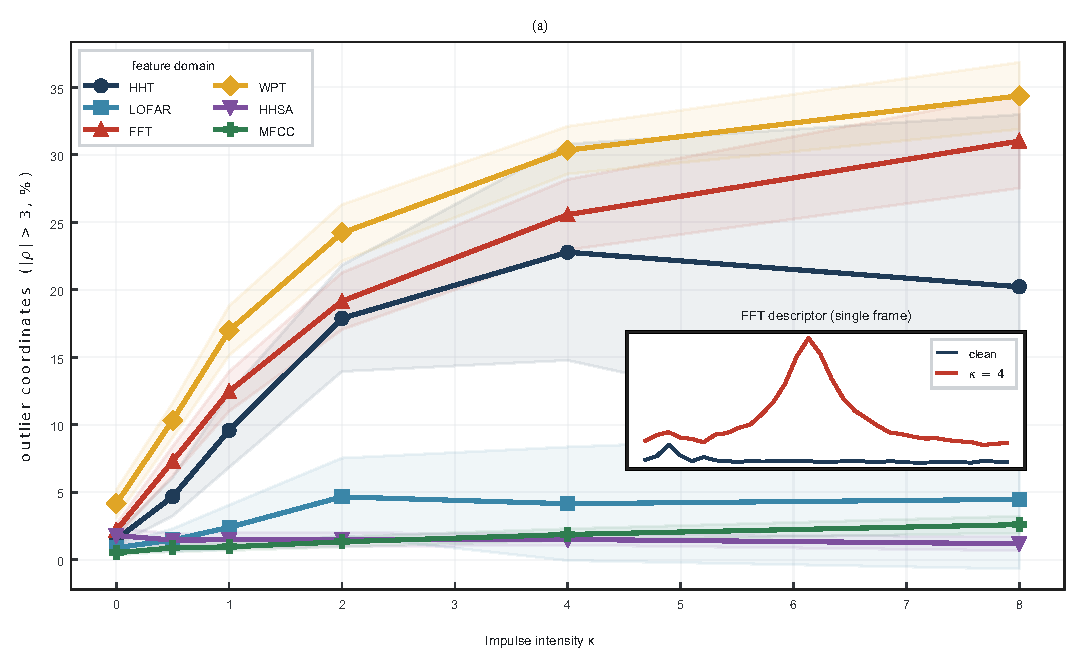
\includegraphics[width=\linewidth]{figures/fig5a.pdf}\\[-0.3em]
  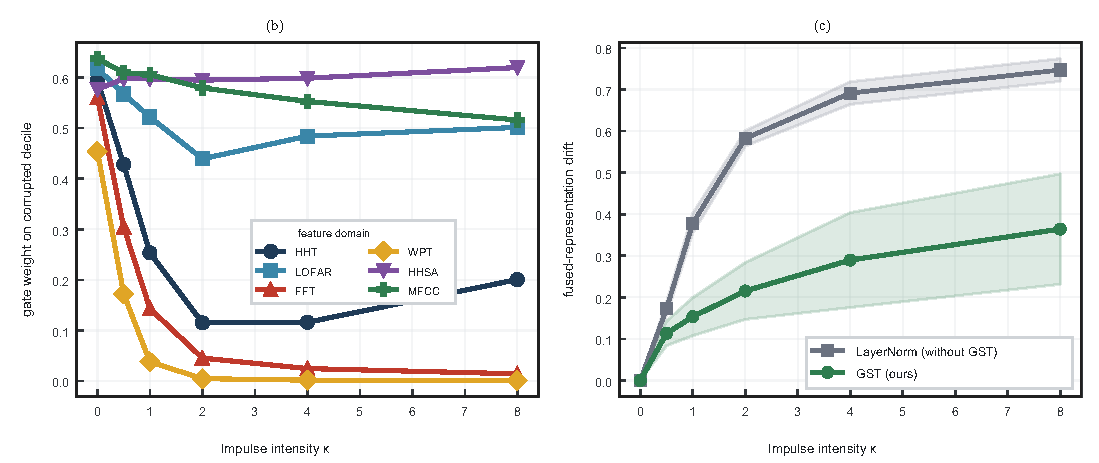
\includegraphics[width=\linewidth]{figures/fig5b.pdf}
  \caption{Impulsive corruption affects the six descriptor domains unequally. Learned reliability weights change selectively, and the corrected fused representation drifts more smoothly from its clean reference than the LayerNorm control in the evaluated range.}
  \label{fig:impulse-app}
\end{figure}

\begin{figure}[h]
  \centering
  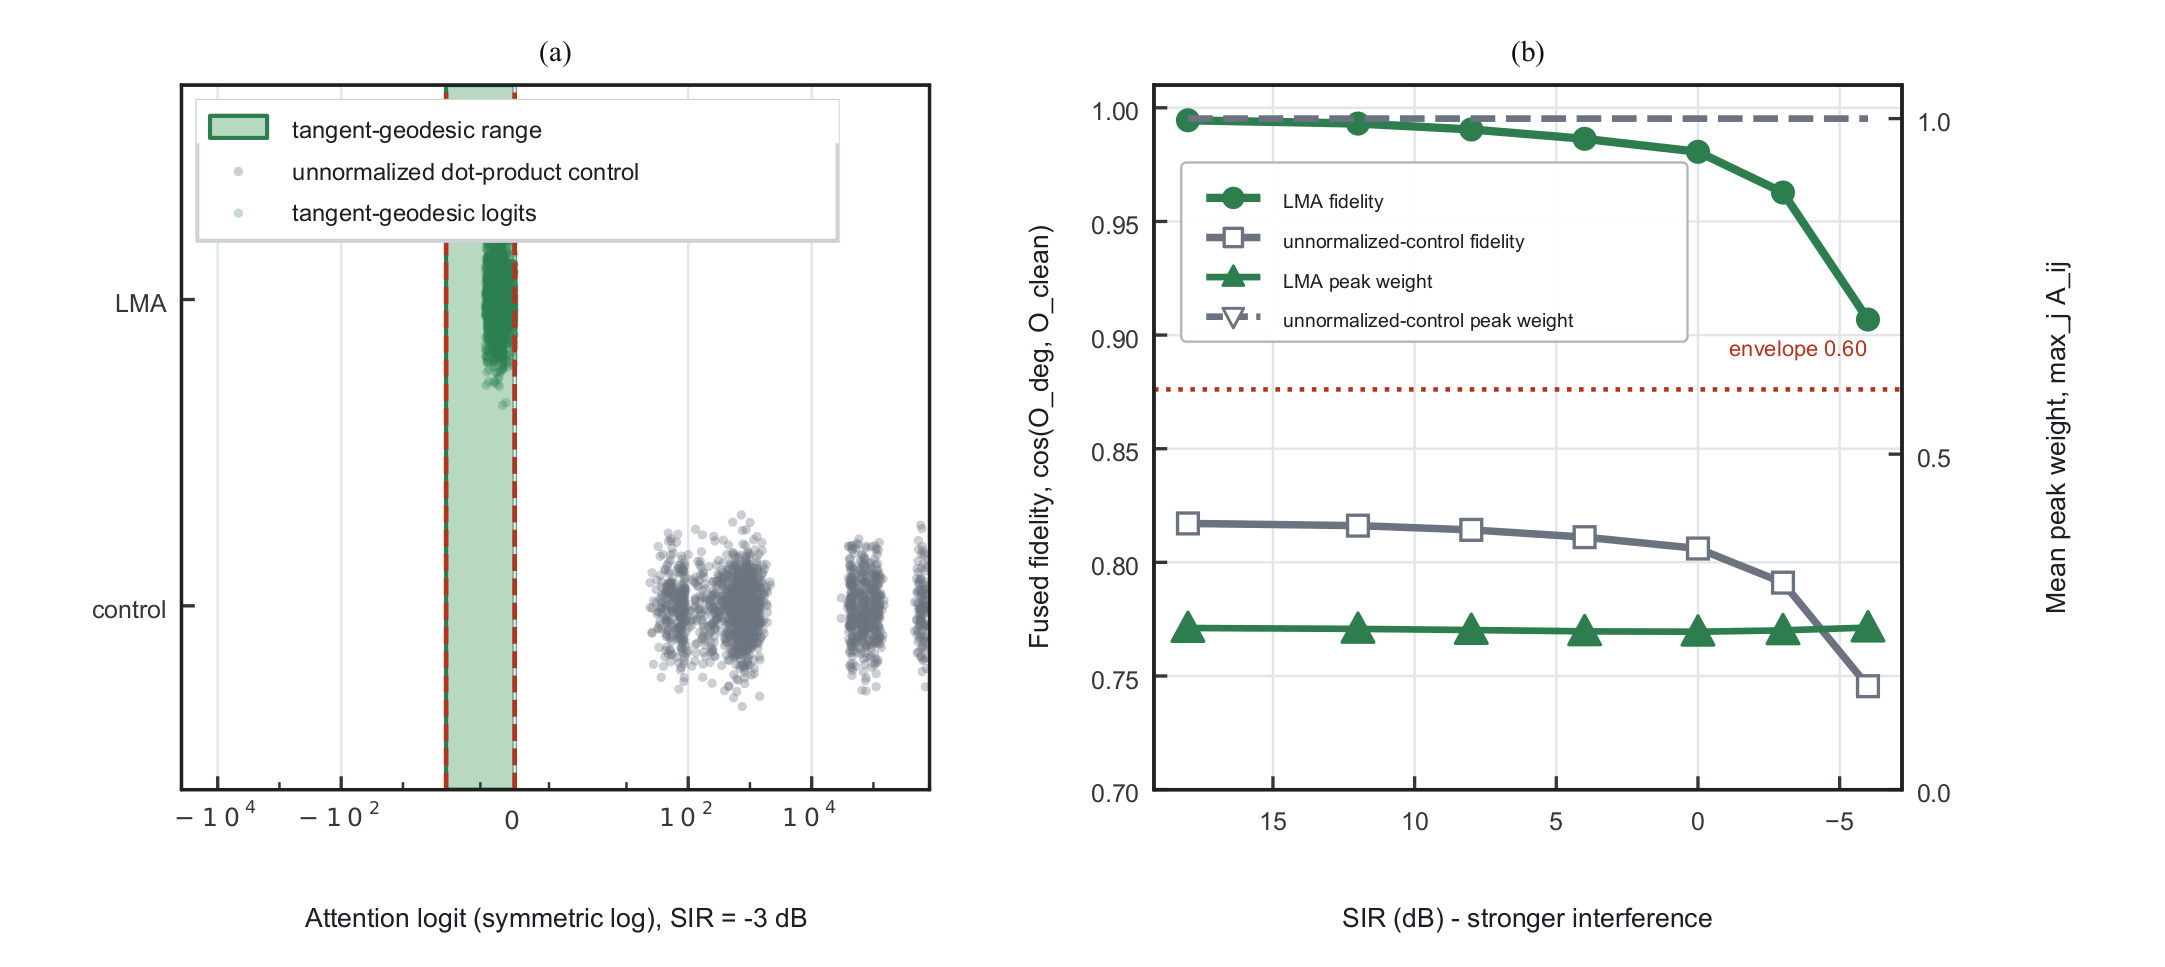
\includegraphics[width=\linewidth]{figures/fig6.png}
  \caption{Tangent-metric attention under co-channel interference. The diagnostic fixes $\gamma=0.50$; normalized projected logits stay within their admissible interval, whereas the unnormalized dot-product control is scale-sensitive.}
  \label{fig:cochannel-app}
\end{figure}

\begin{figure}[h]
  \centering
  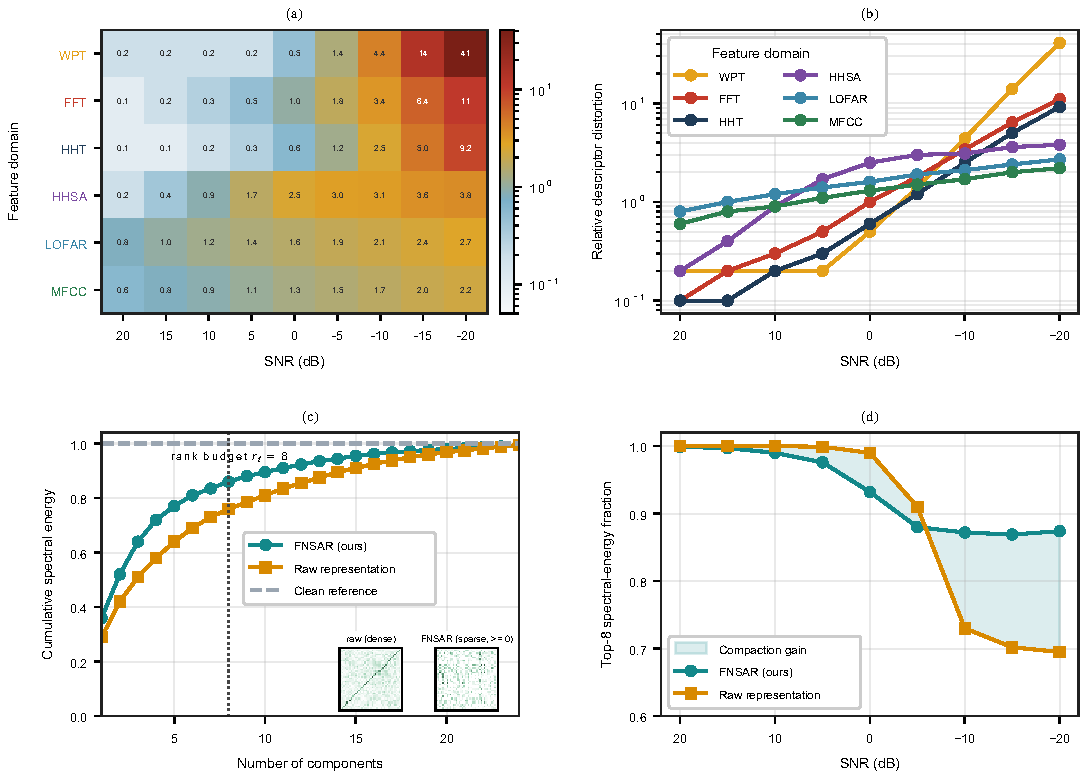
\includegraphics[width=0.94\linewidth]{figures/fig7.pdf}
  \caption{Descriptor sensitivity and factorized sparse temporal-affinity behavior under additive Gaussian noise.}
  \label{fig:noise-app}
\end{figure}

\section{Complete Paired Statistics}

\begin{table}[h]
\caption{Paired Student $t$-tests between RMAL-CRNN and control variants at $0$ dB over the paired multi-seed runs (Holm--Bonferroni corrected). Differences use unrounded paired runs.}
\label{tab:paired-test-app}
\centering
\small
\begin{tabular}{@{}lccccc@{}}
\toprule
Control & Difference & 95\% CI & $t$ & $d_z$ & Holm $p$\\
\midrule
RMA-CRNN & $+1.41$ & $[+0.77,+2.05]$ & $+5.41$ & $+2.05$ & $1.6\times10^{-3}$\\
RL-CRNN & $+1.50$ & $[+1.03,+1.97]$ & $+7.78$ & $+2.94$ & $7.1\times10^{-4}$\\
MAL-CRNN & $+1.80$ & $[+1.20,+2.40]$ & $+7.35$ & $+2.78$ & $7.1\times10^{-4}$\\
CRNN & $+6.96$ & $[+6.69,+7.22]$ & $+63.95$ & $+24.17$ & $3.9\times10^{-9}$\\
\bottomrule
\end{tabular}
\end{table}

\section{Implementation and Sensitivity}
\label{app:implementation}

The selected attention head count is $N_h=4$, factor rank $r_\ell=8$, and fusion dimension $d_f=64$. The learning rate is $10^{-3}$ and batch size is 32. These values come from the repeated scans summarized in Figure~\ref{fig:hyperparameters-app}; the scan characterizes sensitivity around the selected configuration.

All classification results use the benchmark-specific fixed splits and multiple random seeds. We report mean accuracy with sample standard deviation, and paired comparisons use matched runs. Training uses AdamW with learning rate $10^{-3}$ and weight decay $10^{-4}$, cosine learning-rate decay, batch size 32, label smoothing 0.1, gradient clipping at 2, and stochastic weight averaging over the final 30 of 120 epochs. The ablation configuration uses a stratified 60\%/20\%/20\% split with split seed 42.

The full-model parameter count was independently recounted by instantiating the retained PyTorch architecture. It includes the feature pipeline and the CNN--BiLSTM classifier; the parameter count of the proposed modules alone is not the total-model count.
\begin{table}[h]
\caption{Trainable parameter count for the retained ten-class implementation.}
\label{tab:parameter-breakdown}
\centering
\small
\begin{tabular}{@{}lr@{}}
\toprule
Component & Parameters\\
\midrule
GST gates and tangent embeddings & 960\\
LMA, including domain embeddings & 4,388\\
Fusion projection and FNSAR & 13,442\\
CNN--BiLSTM classifier & 320,586\\
\midrule
RMAL-CRNN total & 339,376\\
CRNN control total & 333,322\\
\bottomrule
\end{tabular}
\end{table}
These counts correspond to \texttt{RMALCRNN} and \texttt{BaselineCRNN} in \texttt{ablation.py}. The CRNN has two Conv1D--BatchNorm--ReLU--pool blocks (64/128 channels; kernels 7/3), one bidirectional LSTM (128 hidden units per direction), dropout 0.5, temporal mean pooling, and a linear classifier. The $192\times64$ fusion matrix receives QR initialization and is then trained freely. GST and LMA are implemented by \texttt{StudentTRobustGate}, \texttt{SphericalTangentEmbedding}, and \texttt{LogMapTangentAttention}; FNSAR is \texttt{DiffNSLLR}.

\begin{figure}[h]
  \centering
  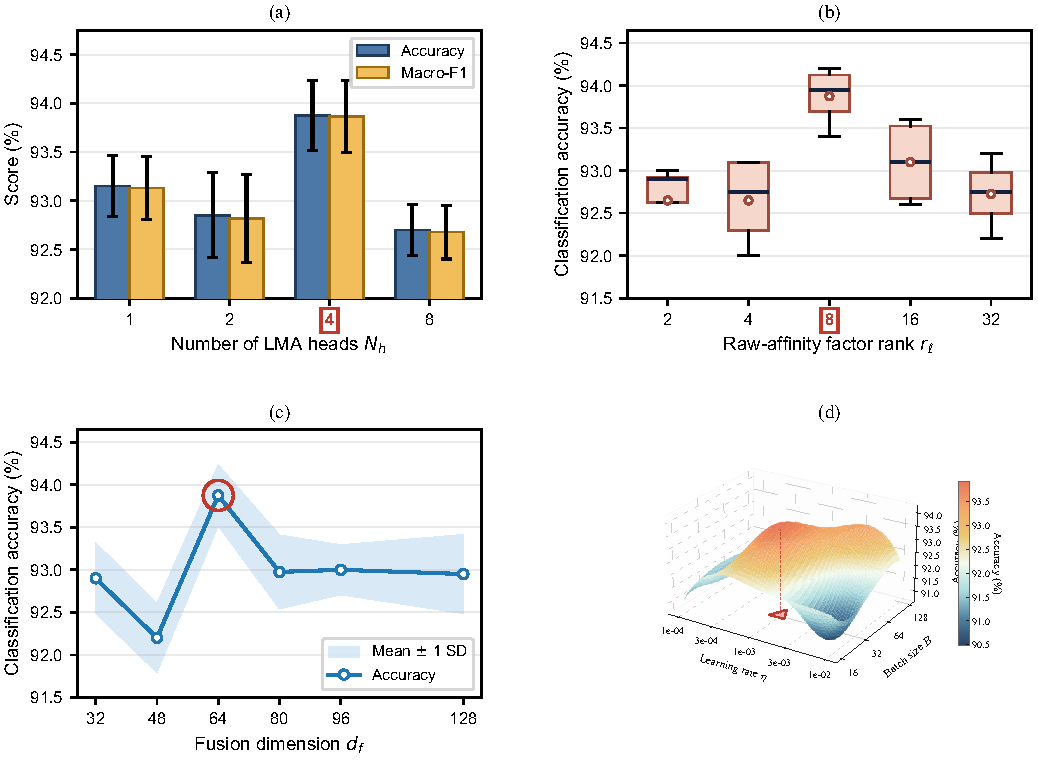
\includegraphics[width=\linewidth]{figures/fig8.pdf}
  \caption{Sensitivity to attention heads, factor rank, fusion dimension, and the learning-rate/batch-size pair.}
  \label{fig:hyperparameters-app}
\end{figure}

The architectures in \texttt{compare.py} are specified directly by their model classes. InceptionTime \citep{fawaz2020inceptiontime} has six Inception modules; CNN-Transformer has two strided Conv1D layers followed by a three-layer, eight-head encoder ($d=128$, feed-forward width 256); SEResNet1D has a convolutional stem and three squeeze-and-excitation residual blocks with channels $(64,128,128)$ \citep{hu2020senet}; TCN uses dilations $(1,2,4,8)$ \citep{bai2018tcn}. SPDNet uses BiMap/ReEig layers and a LogEig classifier \citep{huang2017spdnet}, and BiLSTM uses two bidirectional recurrent layers.

\paragraph{MAtt identity and acoustic adaptation.}
MAtt-A is the acoustic adaptation of the SPD manifold-attention architecture introduced by Pan, Chou, and Wei \citep{pan2022matt} (NeurIPS 2022), implemented as \texttt{MAtt} in \texttt{compare.py}. It has a $192\!\to\!40\!\to\!16$ Conv1D front end, four window-covariance tokens, QR-parameterized BiMap query/key/value maps, Log-Euclidean attention, and a LogEig/vectorization classifier. For SPD queries $\mathbf Q_i$, keys $\mathbf K_j$, and values $\mathbf V_j$, the implemented weights $a_{ij}$ and output $\mathbf O_i$ are
\begin{equation}
a_{ij}=\operatorname{softmax}_{j}\!\left[-|\tau|\sqrt{\|\log\mathbf Q_i-\log\mathbf K_j\|_F^2+10^{-8}}\right],
\qquad \mathbf O_i=\exp\!\left(\sum_j a_{ij}\log\mathbf V_j\right),
\label{eq:matt-adaptation}
\end{equation}
where $\tau$ is a learned scale and matrix log/exp use stabilized eigendecompositions. The acoustic adaptation uses covariance shrinkage 0.3 and diagonal loading $10^{-3}$. The original EEG formulation uses trace-normalized covariance and a different similarity transform, while ManifoldNet is a separate related method.

\paragraph{Additional comparison records.}
TimeMixer++ \citep{wang2025timemixerpp} and MambaSL \citep{jung2026mambasl} are included as sequence-classification baselines. Their formal publications are cited in Table~\ref{tab:comparison}; the MAtt-A acoustic adaptation is specified above.

TimeMixer++ Macro-F1 is $84.00{\pm}1.16$, $89.44{\pm}0.77$, $93.68{\pm}0.60$, and $96.67{\pm}0.49$ at $-5$, $0$, $5$, and $10$ dB. MambaSL Macro-F1 is $82.58{\pm}1.19$, $89.30{\pm}1.05$, $93.20{\pm}0.17$, and $95.97{\pm}0.36$. These results are reported as multi-seed means with sample standard deviations.
